\chapter{Анализ опыта и требований в проектировании энергоэффективных зданий и сооружений в Арктике}
В главе авторы рассматривают опыт Российской Федерации и других стран мира в области проектирования энергоэффективных зданий и сооружений в Арктике и в части требований, предявляемых к таковым.
Задачами анализа является обзор опыта и выявление устойчивых закономерностей в процессах реализации зданий, которые расходуют энергию, реализуя максимальный \gls{factor.usefulEnergy} материалов, изделий, оборудования, механизмов.

При проведении \textbf{оценки}, авторы выделяют следующие оцениваемые аспекты, формирующие структуру анализа:
\begin{itemize}
    \item модельные классы застройки; типологическая классификация объёмно-планировочных решений здания, описываемая процессами,
    которые происходят внутри здания и прилегающей к нему территории (индивидуальное проживание, квартирное проживание, общественно-деловые функции, производство, хранение и т.п.),
    как модельное обощение этой типологии здания;
    \item модельные метрики потребления энергии --- коффициент, который описывает потребление энергии и модельные показатели здания; % TO DO Раскрыть и выявить модель, которую описал И. А. Башмаков. Дополнить при необходимости
    \item методы регулирования --- \gls{law.lna}, группа \gls{law.lna}, стандарты, информационные системы,
    практики и способы вовлечения населения и других владельцев застраиваемых территорий (застройщиков) в процесс разработки и проектирования энергоэффективных зданий.
\end{itemize}

\cite{law_RU_GradoCodex}

% Команды для генерации заголовков в разделе
\providecommand{\scAssesmentHeader}[1]
{\textbf{Оценка опыта и требований в проектировании энергоэффективных зданий #1}}
\providecommand{\scAssesmentBuildingClass}{Модельные классы застройки}
\providecommand{\scAssesmentBuildingMetrics}{Модельные метрики потребления энергии}
\providecommand{\scAssesmentExp}{Опыт применения}
\providecommand{\scAssesmentBuildingLaw}{Методы регулирования}

% Верстка по странам
\section{\scAssesmentHeader{Российской Федерации}}


% \subsection{\scAssesmentBuildingClass}
% % 
% \subsection{\scAssesmentBuildingMetrics}
% 
% ##########-----Регулирование


\subsection{\scAssesmentBuildingLaw}
% 
В части базы обеспечения стандартизацией процессов регулирования энергетической эффективности законодательством России закреплены национальные стандарты,
описывающие нормативные показатели микроклимата \cite{law_RU_RulesCode_BuildingMicroclimateResedentialPublic} с учётом условий от энергетического воздействия внешней среды \cite{law_RU_RulesCode_BuildingClimatology}
и параметры ограждающих конструкций зданий \cite{law_RU_Rules_Code_ThermalPerformance,law_RU_Rules_Code_BuildingEnclosingConstruction}, оптимизация которых позволяет создавать проектные решения построек,
минимизирующие потери тепловой энергии и мероприятия по снижению затрат на обогрев зданий в целом.
В части базы обеспечения методологии законодательство посредством национальных и межгосударственных стандартов определяет принципиальные подходы (на уровне стратегии)
и методики экономической оценки энергетических систем в зданиях.

Основополагающие концепции для принятия решений, связанных c развитием Арктики, исходят из федерального уровня управления и фиксируются в документах стратегического планирования.
Основания разработки нормативно-правовых актов устанавливают Указы Президента РФ или Приказы ведомств.
На период проведения исследования принят Указ Президента РФ от 5 марта 2020 г. N 164 <<Об Основах государственной политики Российской Федерации в Арктике на период до 2035 года>>.
Согласно Указа, устанавливаются такие методы и механизмы регулирования, как:
\begin{itemize}
    \item издание нормативных правовых актов, регулирующих экономическую и иную деятельность в Арктической зоне Российской Федерации;
    \item разработка и реализация стратегии развития Арктической зоны Российской Федерации и обеспечения национальной безопасности на период до 2035 года, стратегии развития арктического туризма в Российской Федерации;
    \item приведение документов стратегического планирования, разработанных в рамках целеполагания, прогнозирования, планирования и программирования на уровне субъекта Российской Федерации, муниципального образования, а также отраслевых документов стратегического планирования в соответствие с настоящими Основами;
    \item создание единой статистической и информационно-аналитической системы в целях осуществления мониторинга социально-экономического развития Арктической зоны Российской Федерации и управления ее социально-экономическим развитием.
\end{itemize}

На федеральном уровне существуют и дополнительно сформированы формализованные структуры, направленные на работу с арктическими территориям:
\begin{itemize}
    \item Министерство иностранных дел Российской Федерации;
    \item Государственная комиссия по вопросам развития Арктики;
    \item Министерство экономического развития России (Департамент развития межрегионального и приграничного сотрудничества);
    \item Комитет по федеративному устройству, региональной политике, местному самоуправлению и делам Севера Совета Федерации Федерального Собрания Российской Федерации;
    \item Совет по Арктике и Антарктике при Совете Федерации Федерального Собрания Российской Федерации;
    \item Комитет по региональной политике и проблемам Севера и Дальнего Востока Государственной Думы ФС РФ;
\end{itemize}
На уровне субъекта Республики Саха (Якутия) авторами установлены следующие формализованные структуры и институции:
\begin{itemize}
    \item Координационный Арктический совет при Главе Республики Саха (Якутия);
    \item Комитет по вопросам коренных малочисленных народов Севера и делам Арктики Государственного Собрания (Ил Тумэн) Республики Саха (Якутия);
    \item Министерство экономики Республики Саха (Якутия) Государственный комитет Республики Саха (Якутия) по делам Арктики.
\end{itemize}
В соответствии с N 190-ФЗ <<Градостроительный кодекс Российской Федерации>> \cite{law_RU_GradoCodex} правовой основой развития территорий являются
документы территориального планирования (Генеральные планы — в случае развития поселений и населённых пунктов),
определяющие стратегию всей административно-территориальной единицы и функциональное назначение территории как класс функциональной зоны,
и документы градостроительного зонирования (Правила землепользования и застройки), устанавливающие правовые возможности и обязанности застройщиков
в форме градостроительных регламентов на предельно допустимые параметры застройки в соответствии с классом территориальной зоны.

В соответствии с № 261-ФЗ <<Об энергосбережении и о повышении энергетической эффективности и о внесении изменений в отдельные законодательные акты Российской Федерации>>
\cite{law_RU_fz_EnergyEff}, ст. 6, допускается передача полномочий органов государственной власти на региональный уровень. При этом органы власти на уровне субъектов и на уровне местного
самоуправления уполномочены разрабатывать собственные программные документы в области энергоэффективного строительства.

Стандарты по развитию ориентированной на человека среды в насёленных местах, в частности --- в городах, --- на период проведения исследования находятся в разработке.
Публичная версия по завершении разработки будет доступна для ознакомления потенциальным инвесторам и интересантам развития территории \cite{law_RU_govAggregatorArcticStandart}.
Разработку «арктического стандарта» ведет АНО «Информационно-аналитический центр
Государственной комиссии по вопросам развития Арктики» под кураторством Минвостокразвития России и Минстроя России.
Техническая реализация представляет комплекс документов, в котором определены основные принципы и подходы к формированию
комфортной городской среды в соотвествии с потребностями и запросами местных жителей, с учётом климатических условий и особенностей социально-экономического развития городов Арктики.
Эти стандарты также нацелены на комплексный подход со включением опыта строительства и объёмно-планировочных решений из традиционных способов возведения северного дома,
которые с течением времени были апробированы и оптимизированы в части энергоэффективности.

В Российской Федерации с начала 90-х годов прошлого столетия начали серьезно заниматься созданием новой нормативно-правовой базы для повышения энергоэффективности зданий и
в 1995 году впервые было введено нормирование приведенного сопротивления теплопередаче ограждающих конструкций в зависимости от градусо-сутки отопительного периода
и введены изменения в СНиП II-3-79* <<Строительная теплотехника>> \Code{[14]}.

Повышение требований по тепловой защите зданий разделили на два этапа: 1998-2000 гг. и 2001-2005 гг.
Для примера в Таблице \ref{tab:method_gsop_phases} приведены требуемые значения приведенного сопротивления теплопередаче стен, цокольного перекрытия и окон для жилых зданий в условиях г. Якутска.
Также 3 апреля 1996 г. был принят Федеральный закон от N 28-ФЗ "Об энергосбережении" и началась реализация федеральной целевой программы "Энергосбережение России" на 1998 - 2005 годы.
% \begin{equation}
%     R_\text{огрконструкции}^\text{требуемое}\text{, м}{^2} \times \text{°С/Вт}
% \end{equation}

\begin{center}
    \begin{longtable}{|m{0.26\textwidth}|c|c|c|}
        \caption{Требуемые значения приведенного сопротивление теплопередаче конструкций для многоквартирных зданий в г.Якутске по СНиП II-3-79* <<Строительная теплотехника>> с изменениями № 3}
        \label{tab:method_gsop_phases}
        \\ \hline
        \multirow{2}{8cm}{ГСОП, \textdegree C$\times$сут\slash год} & \multicolumn{3}{c|}{$R_\text{огрконструкции}^\text{требуемое}\text{, м}{^2} \times \text{°С/Вт}$}\\
        \cline{2-4}
        & Стены & Покрытия, цокольное перекрытие & Окна \\
        \hline \endfirsthead
        \subcaption{Продолжение таблицы~\ref{tab:method_gsop_phases}}
        \\ \hline \endhead
        \hline \subcaption{Продолжение на след. стр.}
        \endfoot
        \hline \endlastfoot
        1 этап & 2,91 & 4,80 & 0,76             \\
        \hline
        2 этап & 5,09 & 7,48 & 0,76             \\
        \hline
    \end{longtable}
\end{center}

В 2003 г. введен в действие СНиП 23-02-2003 <<Тепловая защита зданий>> \cite{law_RU_Rules_Code_ThermalPerformance} и в нем предусмотрен дополнительно комплексный подход, заключавшийся в ограничении затрат тепла на отопление и вентиляцию. При выполнении указанных условий разрешалось некоторое ослабление требований к отдельным ограждающим элементам. 
В ноябре 2009 года принят Федеральный закон №261 <<Об энергосбережении и о повышении энергетической эффективности…>> \cite{law_RU_fz_EnergyEff}.
В соответствии с этим законом, предусмотрено снижение энергоемкости ВВП России на 40\% к 2020 году и в 2.5. – 3 раза к 2030 году (относительно уровня 2007 года).
В дальнейшем НИИСФ РААСН проведены научно-прикладные работы по гармонизации российских норм по тепловой защите зданий с аналогичными зарубежными нормами развитых стран \Code{[16]}.
В настоящее время оценка новой нормативно-правовой базы показала, что Россия серьезно улучшила позицию в рейтинге среди стран по реализации политики энергоэффективности.
При проектировании тепловой защиты зданий и сооружений \Code{[17]}.

Главным регламентирующим документом выступает СП 50.13330.2012 <<Тепловая защита зданий. Актуализированная редакция СНиП 23-02-2003>> \cite{law_RU_Rules_Code_ThermalPerformance}.
Основные характеристики климата района строительства объектов определяются по СП 131.13330.2020 <<Актуализированная редакция СНиП 23-01-99* Строительная климатология>> \cite{law_RU_RulesCode_BuildingClimatology}.
Основные параметры микроклимата в помещениях зданий регламентируются ГОСТ 30494-2011 <<Здания жилые и общественные. Параметры микроклимата в помещениях>> \cite{law_RU_RulesCode_BuildingMicroclimateResedentialPublic}.

В строительных нормах СП 50.13330.2012 \cite{law_RU_Rules_Code_ThermalPerformance} установлены требования к:
\begin{itemize}
    \item приведенному сопротивлению теплопередаче ограждающих конструкций здания;
    \item удельной теплозащитной характеристике здания;
    \item ограничению минимальной температуры и недопущению конденсации влаги на внутренней поверхности ограждающих конструкций в холодный период года, за исключением светопрозрачных конструкций с вертикальным остеклением (с углом наклона заполнений к горизонту 45° и более);
    \item теплоустойчивости ограждающих конструкций в теплый период года;
    \item воздухопроницаемости ограждающих конструкций;
    \item влажностному состоянию ограждающих конструкций;
    \item теплоусвоению поверхности полов;
    \item расходу тепловой энергии на отопление и вентиляцию зданий.
\end{itemize}


% Рассмотрим некоторые требования из них относительно жилых зданий, строящихся в арктических районах Республики Саха (Якутия). 
% Для проектирования тепловой защиты в соответствие с СП 50.13330.2012 \cite{law_RU_Rules_Code_ThermalPerformance} определяется основной показатель - градусо-сутки отопительного периода (1) в зависимости от места расположения объекта строительства:

\begin{eqndesc}
    \begin{equation}\label{eq:gsop}
        \text{ГСОП}=\ (t_{\text{внутр}}-t_{\text{отпериода}})\times z_{\text{отпериода}}
    \end{equation}

    где $t_{\text{внутр}}$ — расчётная температура внутреннего воздуха, °С,\\
    $t_{\text{отпериода}}$ — средняя температура периода со средней суточной температурой воздуха ниже или равной 8°С (в соответствии с положениями \cite{law_RU_RulesCode_BuildingClimatology}),\\
    $z_{\text{отпериода}}$ — продолжительность (в сутках) периода со средней суточной температурой воздуха ниже или равной 8°С (в соответствии с положениями \cite{law_RU_RulesCode_BuildingClimatology}).
\end{eqndesc}

% ГСОП=(t_в-t_от)×z_от,           (1)
% где t_в – расчетная температура внутреннего воздуха здания, °С;
% t_от, z_от - средняя температура наружного воздуха, °С, и продолжительность, сут/год, отопительного периода.


В настоящее время в России используется следующая классификация энергоэффективности зданий:
рейтинг энергоэффективности здания представлен латинскими буквами A++, A+, A, B+, B, C+, C, C-, D, E, где «A++» представляет наивысший рейтинг,
«C» обозначает обычный уровень, а «E» выражает низший уровень.  Данная классификация регламентируется СП 50.13330.2012 Тепловая защита зданий \cite{law_RU_Rules_Code_ThermalPerformance}
и используется при получении энергетического паспорта здания в Российской Федерации. При этом следует отметить, что  согласно п.10.5 \cite{law_RU_Rules_Code_ThermalPerformance},
присвоение зданию класса "В" и "А" производится только при условии включения в проект следующих обязательных энергосберегающих мероприятий:
\begin{itemize}
    \item устройство индивидуальных тепловых пунктов, снижающих затраты энергии на циркуляцию в системах горячего водоснабжения и оснащенных автоматизированными системами управления и учета потребления энергоресурсов, горячей и холодной воды;
    \item применение энергосберегающих систем освещения общедомовых помещений, оснащенных датчиками движения и освещенности;
    \item применение устройств компенсации реактивной мощности двигателей лифтового хозяйства, насосного и вентиляционного оборудования.
\end{itemize}

Кроме в России приняты ряд стандартов, касающихся обеспечения энергетической эффективности зданий.
ГОСТ Р 54862-2011 \Code{[29]} устанавливает метод определения минимальных требований к функциям систем автоматизации
(далее BACS – building automation and control systems) и технического управления зданий (TBM - technical building management),
которые должны внедряться в зданиях различного назначения; методы оценки влияния указанных функций на потребление энергии зданием,
позволяющие ввести характеристики влияния этих функций в расчеты параметров энергетической эффективности зданий.
В данном стандарте подробно приведены функции управления подсистемами: отоплением, вентиляцией и кондиционированием, освещением, системой автоматизации квартир и всего дома, эксплуатацией и технического обслуживания квартир и всего здания в соответствии классам энегоэффективности зданий.
Кроме того, действуют несколько стандартов, оценивающих экономическую эффективность принимаемых в проекте мероприятий.
ГОСТ 56295-2014 \Code{[30]} и ГОСТ 56502-2015 \Code{[31]} устанавливают требования и правила расчетов экономической эффективности
вариантов энергосберегающих мероприятий в зданиях и выбора наиболее целесообразного варианта реализации таких мероприятий.
Таким образом, повышенные требования по тепловой защите зданий обязывает использование энергоэффективных материалов и технологий при строительстве малоэтажных жилых домов
в арктических районах, и ставит задачу для разработки новых конструктивных решений наружных ограждений.
Однозначно, чтобы достичь требуемые значения сопротивления теплопередаче в наружных ограждающих конструкциях, в первую очередь,
необходимо применять современные теплоизоляционные материалы с низким коэффициентом теплопроводности.
Следует отметить, что в арктических районах республики с учетом высоких расходов на отопление зданий необходимо проектировать жилые дома с высоким классом энергосбережения.


Таким образом, акцент регулирования энергоэффективного строительства в Российской Федерации смещён на регулирование посредством механизмов распределения полномочий в соответствии с принципами
местного самоуправления и разработку методических указаний, которые позволят сформировать базу знаний для внедрения в процесс строительства у разнообразных категорий застройщиков.



% ##########-----Опыт


\subsection{\scAssesmentExp}
% 
В Россиской Федерации продолжаются поиский энергетически эффективных подходов в проектировании объёмно-планировочных решений зданий.
Наибольшее влияние на этот процесс оказали разработки В. Щипкова, Б. М. Полуя \cite{1989up_Poluyi_ArchGradoVsurovomKlimate}, К. Г. Туралысова \cite{1996up_Turalysov_BiospherRasseleniye},
труды которых обобщают подходы коренного населения, выработанные при проживании на арктических территориях,
с промышленнными задачами, формирующими требования к расселению, которые были актуальными на период начала промышленного освоения Севера.
В части организации застройки описанные в этих концепциях принципы компактности остаются востребованными и применимыми для формирования энергосберегающей застройки (Рисунок. \ref{fig:st1ch03_ruexp_003}).
\clearpage
\begin{figure}
    \centering
    \includegraphics[width=\textwidth]{assets/figures/st1ch03_ruexp_001.png}
    \caption{Концепция компактной энергосберегающей застройки на Севере. Блокированная застройка частными домами}
    \label{fig:st1ch03_ruexp_001}
  \end{figure}

% \clearpage

Принципы энергосберегающей планировки, которые иллюстрируют Рисунки \ref{fig:st1ch03_ruexp_001}, \ref{fig:st1ch03_ruexp_004}, \ref{fig:st1ch03_ruexp_005}, \ref{fig:st1ch03_ruexp_006}, \ref{fig:st1ch03_ruexp_007},
разрабатываемые в рамках концепций застройки, реализуются при вахтовом расслении, на военных базах (Рисунок \ref{fig:st1ch03_ruexp_002}) и научных станциях.


\begin{figure}
    \centering
    \includegraphics[width=\textwidth]{assets/figures/st1ch03_ruexp_003.png}
    \caption{Уменьшение площади ограждающих конструкций посредством компактной формы постройки в индивидуальном частном домостроении}
    \label{fig:st1ch03_ruexp_003}
  \end{figure}
% \clearpage

\begin{figure}
    \centering
    \includegraphics[width=\textwidth]{assets/figures/st1ch03_ruexp_004.png}
    \caption{Концепция компактной энергосберегающей застройки на Севере. Квартирные дома}
    \label{fig:st1ch03_ruexp_004}
  \end{figure}
% \clearpage


\begin{figure}
    \centering
    \includegraphics[width=\textwidth]{assets/figures/st1ch03_ruexp_005.png}
    \caption{Концепция компактной энергосберегающей застройки на Севере. Вахтовое расселение}
    \label{fig:st1ch03_ruexp_005}
  \end{figure}


\begin{figure}
    \centering
    \includegraphics[width=\textwidth]{assets/figures/st1ch03_ruexp_006.png}
    \caption{Концепция компактной энергосберегающей застройки на Севере. Планировочные решения жилого блока}
    \label{fig:st1ch03_ruexp_006}
  \end{figure}


\begin{figure}
    \centering
    \includegraphics[width=\textwidth]{assets/figures/st1ch03_ruexp_007.png}
    \caption{Концепция компактной энергосберегающей застройки на Севере. Экранирующая противоветровая застройка районов}
    \label{fig:st1ch03_ruexp_007}
  \end{figure}

% \clearpage
\begin{figure}
  \centering
  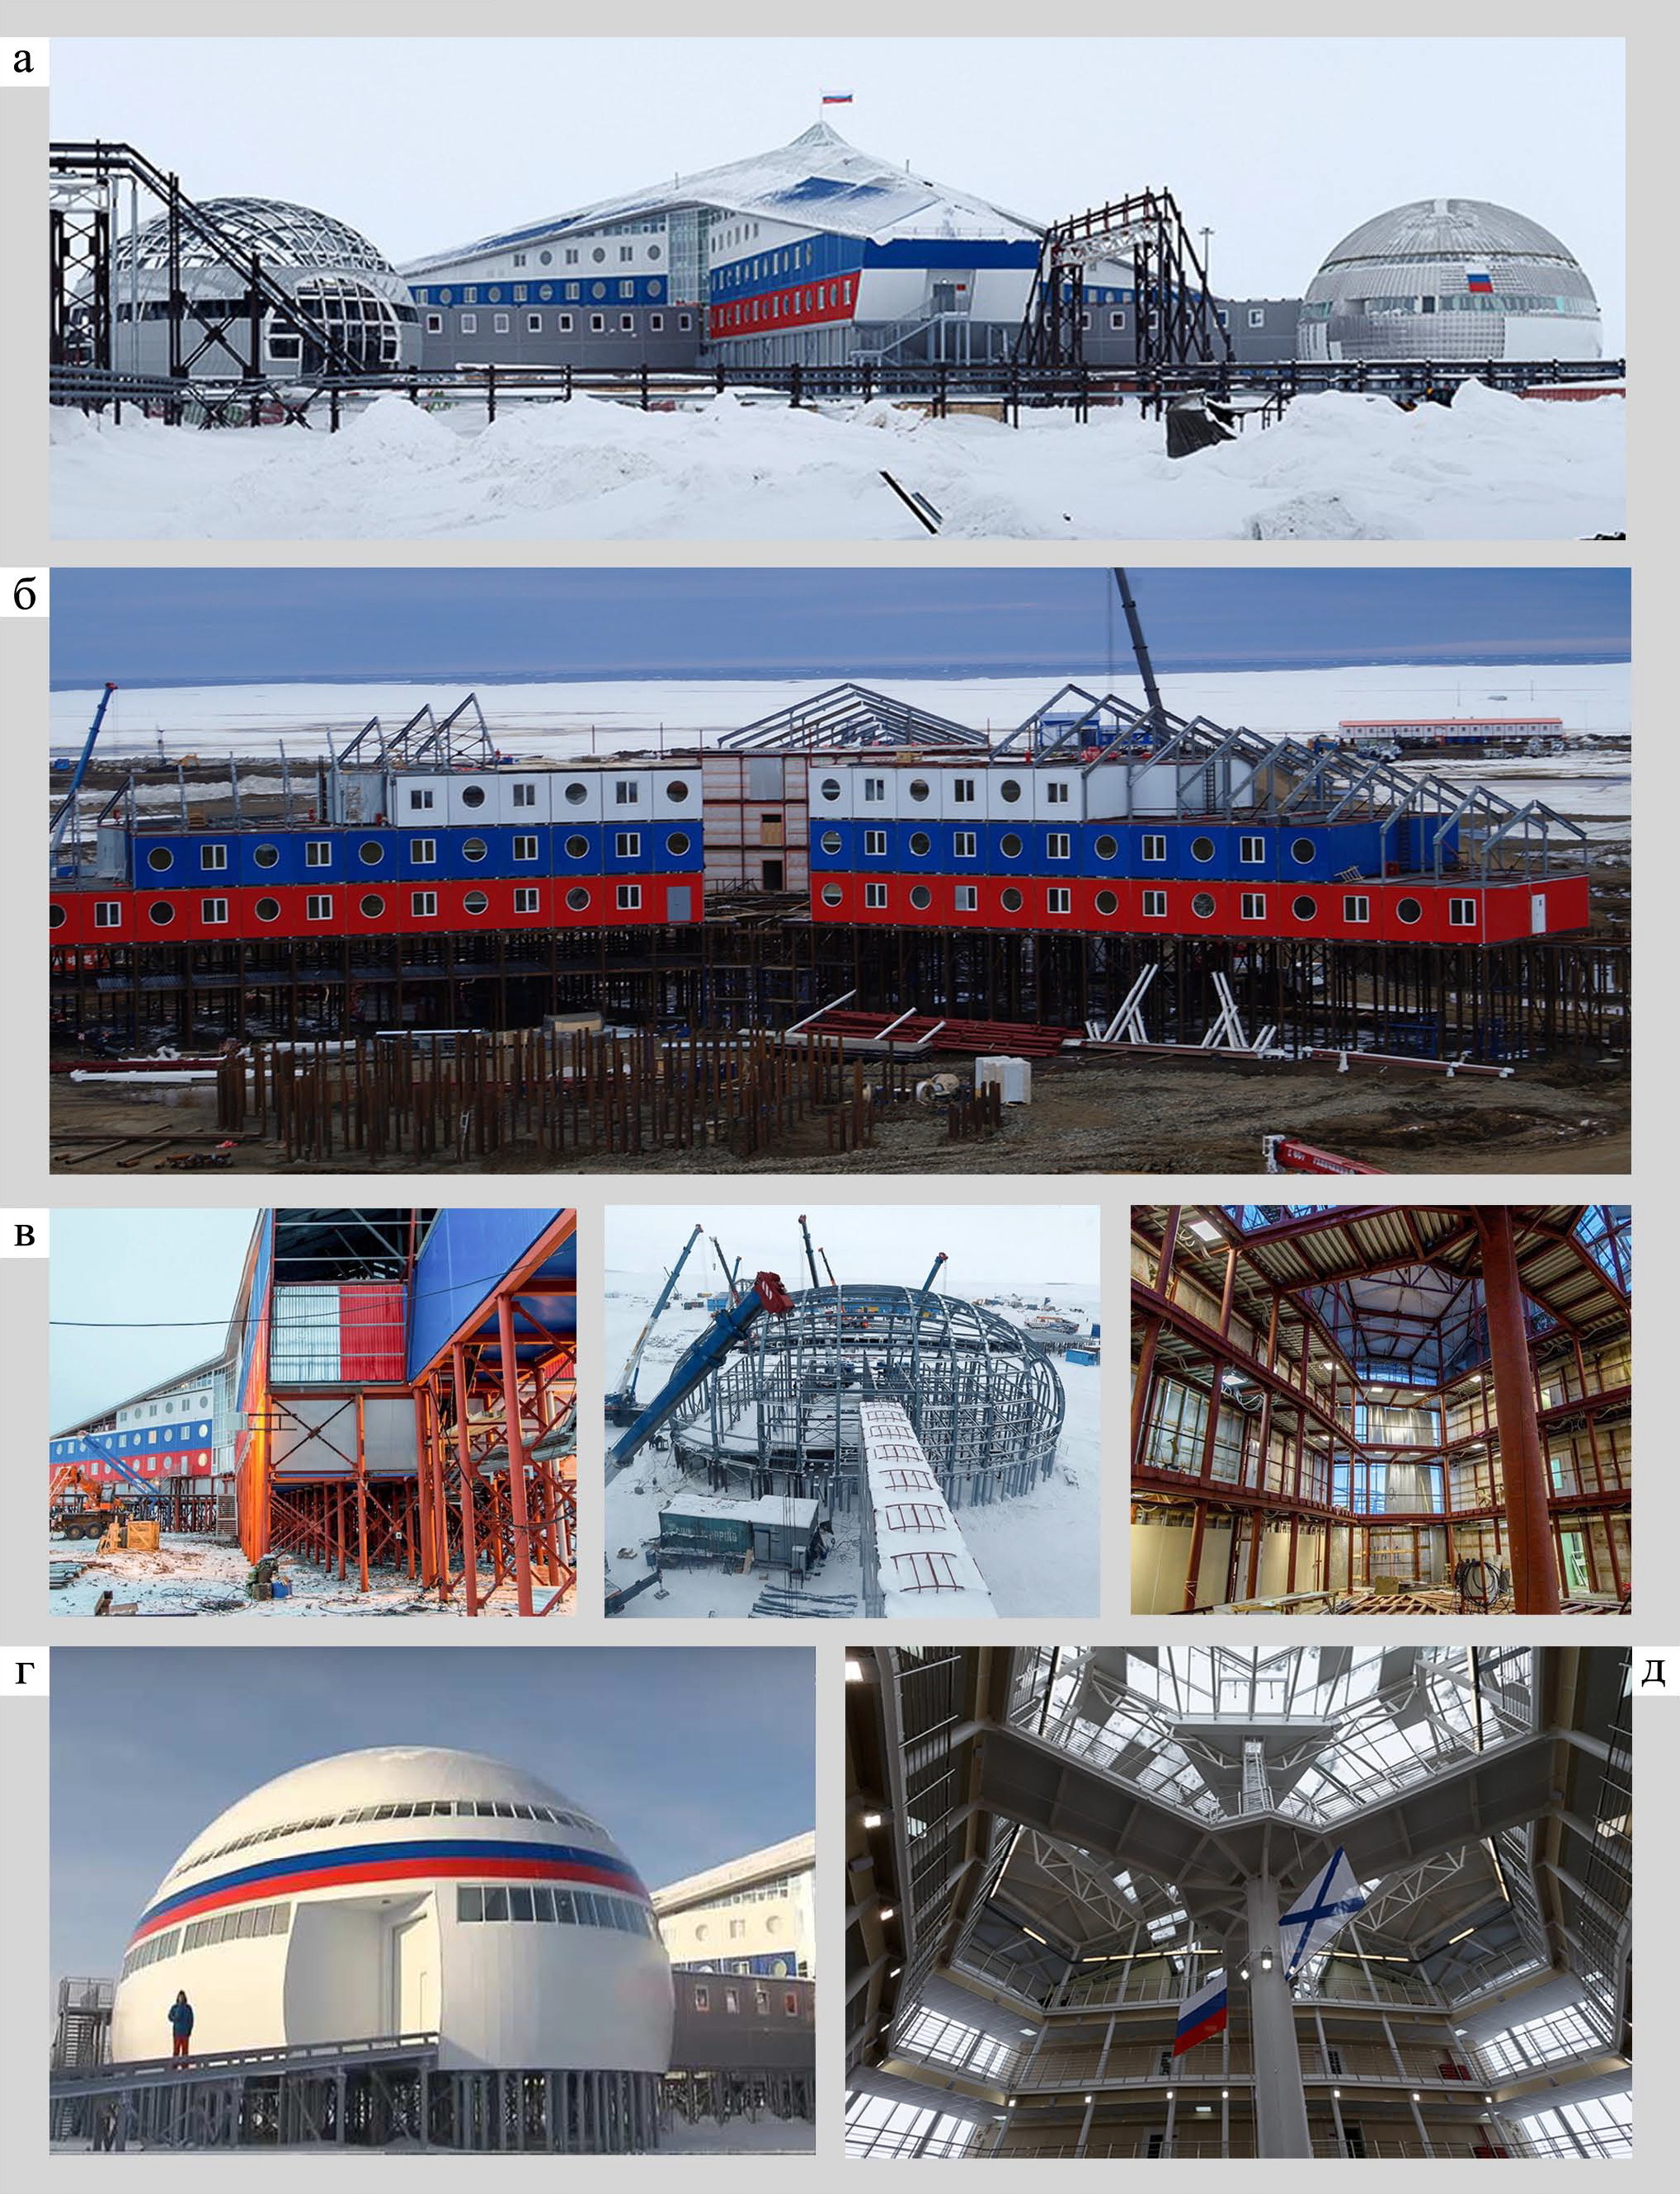
\includegraphics[width=\textwidth]{assets/figures/st1ch03_ruexp_002.png}
  \caption{Российская военная база <<Арктический трилистник>> на острове Земля Александры (архипелаг Земля Франца Иосифа):
  а - Общий вид военной базы; б, в - Конструктивные особенности военной базы; г - Один из трех эллипсоидных объемов военной базы; д - Интерьер военной базы}
  \label{fig:st1ch03_ruexp_002}
\end{figure}

\begin{figure}
    \centering
    \includegraphics[width=\textwidth]{assets/figures/st1ch03_ruexp_008.png}
    \caption{Вахтовый поселок месторождения Купол, Чукотский автономный округ}
    \label{fig:st1ch03_ruexp_008}
  \end{figure}


\begin{figure}
    \centering
    \includegraphics[width=\textwidth]{assets/figures/st1ch03_ruexp_009.png}
    \caption{Вахтовый поселок месторождения Эбелях-Гусиный, Анабарский улус. Республика Саха (Якутия)}
    \label{fig:st1ch03_ruexp_009}
  \end{figure}


\begin{figure}
    \centering
    \includegraphics[width=\textwidth]{assets/figures/st1ch03_ruexp_010.png}
    \caption{Вахтовый поселок Сабетта, Ямало-Ненецкий автономный округ}
    \label{fig:st1ch03_ruexp_010}
  \end{figure}


\section{\scAssesmentHeader{Соединённых Штатов Америки}}


\subsection{\scAssesmentBuildingClass}
% 
\subsection{\scAssesmentBuildingMetrics}
% 
\subsection{\scAssesmentBuildingLaw}


\section{\scAssesmentHeader{Норвегии}}


% \subsection{\scAssesmentBuildingClass}
% % 
% \subsection{\scAssesmentBuildingMetrics}

% ##########-----Регулирование


\subsection{\scAssesmentBuildingLaw}
% 
Регулирование вопросов энергоэффективности строительства в Норвегии закладывает основы на уровне законодательства о природопользовании.
С целю унификации процесса издаются методические материалы \cite{law_NORW_RulesCode_Natureuse} для владельцев земель и широкого круга участников градостроительной деятельности, включая частных застройщиков.


Kommuneplanes\footnote{Общинная (Коммуны являются вторым административным уровнем деления Норвегии после губерний  — фюльке)
            социальная часть плана определяет общие долгосрочные цели для сообщества Тромсё и муниципалитета Тромсё на двенадцатилетнюю перспективу и является стратегиейдля достижения этих целей.
            На этом уровне применяется механизм соучаствующего проектирования, частью которого являются публичные информационные системы (географический портал, сайт администрации общины),
            использующиеся в публичных обсуждениях и на ранних этапах принятия решений.
            На раннем этапе производится консультация с интересантами территории (преимущественно, это жители и владельцы предприятий)}
являются документами территориального планирования муниципального уровня, состоящих из социальной и землеустроительной частей муниципального генерального плана.
Ресурс www.gatami.no является порталом-агрегатором принятия решений, с помощью которого любой интересант, включая жителей,
может сообщать о проблемах и формировать запросы на развитие территории, а управленческая команда — получать оперативную информацию и проводить оперативную аналитику
и реагирование на ситуации. Прикладные информационные технологии позволяют создавать формы для пользователей и унифицировать структуры поступающих данных без создания избыточных юридически формализованных форм стандартизации. В свою очередь, унифицированная структура позволяет произвести автоматизированную обработку методами статистики, создавать визуализацию данных для управленческих команд и, как итог, повышать качество обратной связи и оперативность в принятии решений.
Представляющие ценность исторические здания являются предметом охраны местного законодательства об объектах культурного наследия.
Портал https://tromso.gravearbeider.no/ на базе геоинформационной платформы позволяет отслеживать заявки на археологические исследования территории застройки.

% ##########-----Опыт


\subsection{\scAssesmentExp}

\section{\scAssesmentHeader{Финляндии}}


% \subsection{\scAssesmentBuildingClass}
% % 
% \subsection{\scAssesmentBuildingMetrics}

% ##########-----Регулирование


\subsection{\scAssesmentBuildingLaw}
% 
Политика на уровне государства направлена на обеспечение мер по преодолению грядущего глобального энергетического кризиса,
государство видит национальную безопасность основой бесперебойных поставок энергии и, в свою очередь, энергию ---
как основу общества и его развития для будущего \cite{law_FIN_govMinEnvSecurity}. Эта позиция находит отражение как основополагающее направление в домостроении.

Большинство финнов живут в частных домах. Одним из основных преимуществ жилья, занимаемого владельцем, по сравнению с арендованным жильем является то,
что часть расходов на жилье, например, взносы по ипотеке, может учитываться как сбережения.

Ministry of the Environment\footnote{рус. Министерство окружающей среды} ведает полномочиями и правовыми актами,
регулирующими взаимодействие человека и жилой среды. Цель министерства окружающей среды заключается в обеспечении адекватного предложения различных видов жилья на рынке жилья,
направлении строительной отрасли и жилищного строительства в направлении, которое является экологически устойчивым, и расширении возможностей жителей влиять на свои жилищные условия.
В министерстве окружающей среды ответственность за жилищное строительство возложена на Департамент антропогенной среды.
Субсидии, субсидии и гарантии, связанные с жильем и строительством, предоставляются Центром финансирования и развития жилищного строительства Финляндии (АРА),
который также руководит и контролирует использование субсидируемого государством строительного фонда АРА.

На уровне субъекта (региональном) действует Regional plan and land use planning, регламентируемый The Land Use and Building Act 132/1999 28 §\footnote{рус. Закон о землепользовании и строительстве},
устанавливющий требования к содержанию регионального плана \cite{law_FIN_RulesCode_LanduseAndBuilding}.
Региональное планирование включает в себя: региональную схему, региональный план, программу регионального развития.
Региональный план представляет собой карту, подготовленную в соответствии с Законом о землепользовании и строительстве, отображающую планы землепользования и структуры общин региона.
В нем описывается строительство и экологическое развитие в ближайшие десятилетия. Региональный план содержит инструкции по муниципальному планированию землепользования и другим официальным мероприятиям, которые влияют на землепользование.
Региональные планы составляются и утверждаются областными советами.
Несколько факторов влияют на муниципальную политику землепользования (планы землепользования и земельная политика).
К ним относятся фактические процессы планирования землепользования и другие виды планирования землепользования, а также промышленная, социальная и жилищная политика.
К числу инструментов планирования землепользования муниципалитетов относятся следующие:
\begin{itemize}
    \item стратегии и программы землепользования в муниципалитете;
    \item местный генеральный план и местный план территории;
    \item земельная политика;
    \item постановление о строительстве.
\end{itemize}
Региональный план определяет, как земля используется в регионе. Местный генеральный план устанавливает цели землепользования в муниципалитете.
В нем излагается общее развитие муниципалитета и использование земельной площади, которую он охватывает, например, расположение жилых районов, мест работы и транспортных маршрутов.
Можно подготовить частичный генеральный план для таких районов, как берега. Такой план может быть более подробным, чем местный генеральный план.
Каждый муниципалитет несет ответственность за подготовку местного генерального плана.
Этот план утверждается муниципальным советом. Если муниципалитеты подготовят общий местный генеральный план, он будет утвержден общим органом муниципалитетов и утвержден министерством окружающей среды.
Закон о землепользовании и строительстве устанавливает требования к содержанию местного генерального плана.
Местный генеральный план используется в качестве основы для подготовки местных подробных планов.


Сбор обратной связи от интересантов территории в ходе разработки документов на всех уровнях принятия решений осуществляется средствами государственных информационных систем
и георафических порталов. В настоящее время в финском государственном управлении проводятся широкомасштабные реформы, направленные на совершенствование управления информацией
и ее использования. Благодаря этим реформам информация, содержащаяся в различных регистрах центральных и местных органов власти, будет соответствовать международным стандартам и
будет более функционально совместимой и пригодной для использования, чем раньше. За информацию о антропогенной среде отвечает главным образом министерство окружающей среды.
Цифровизация административного сектора осуществляется в министерстве в рамках двух широких образований.
Цель состоит в том, чтобы создать основу для общенациональных электронных услуг в сфере недвижимости и строительства, а также для новых возможностей для бизнеса.
Другим аспектом работы в области развития является функциональная совместимость информации о антропогенной среде, поощряемая широкой группой по сотрудничеству.
Вторым объектом является четырехлетний проект Ryhti, который готовит общенациональную информационную систему для антропогенной среды.
Эта работа изложена в Законе о землепользовании и строительстве, который в настоящее время пересматривается.
В его основные задачи входит повышение качества строительства и содействие цифровизации.


Таким образом, регулирование вопросов энергоэффективности зданий Финляндии органично включено в структуру законодательства и реализуется как системный подход,
связанный с территориальным планированием и управлением развитием территориями. Технологии информационного моделирования тесно интегрируются с сообществом и застройщиками,
позволяя реализовать комплексные подходы к оценке и оптимизации параметров энергопотребления зданий при застройке.

% ##########-----Опыт


\subsection{\scAssesmentExp}

Большинство финнов живут в частных домах. Одним из основных преимуществ жилья, занимаемого владельцем, по сравнению с арендованным жильем является то,
что часть расходов на жилье, например, взносы по ипотеке, может учитываться как сбережения. Однако покупка дома обычно влечет за собой получение кредита,
что делает его существенным и долгосрочным. срочное экономическое обязательство, требующее тщательного рассмотрения.
% \clearpage
\begin{figure}
    \centering
    \includegraphics[width=\textwidth]{assets/figures/st1ch03_finexp_001.png}
    \caption{Социальное крупнопанельное жильё в Финляндии (фотоснимок из ресурса https://iti-consulting.ru/dostupnoe-zhile-finskij-opyt-foto/)}
    \label{fig:st1ch03_finexp_001}
  \end{figure}


В крупных населённых пунктах Арктики, таких как Оулу, преобладает микрорайнная застройка блокированными секциями в виде линейных и перемитральных фронтов застройки,
реализуемая с целью компактного распределения инженерных сетей и энергосбережения посредством предотвращения потерь тепла.
Эти объекты возводятся с применением железобетонных каркасов и крупнопанельных модулей (Рисунок \ref{fig:st1ch03_finexp_001}).


